\documentclass[11pt,a4paper]{article}

\usepackage[margin=1in]{geometry}
\usepackage[T1]{fontenc}
\usepackage{lmodern}
\usepackage{microtype}
\usepackage{graphicx}
\usepackage{subcaption}
\usepackage{amsmath}
\usepackage{booktabs}
\usepackage{hyperref}
\usepackage{xcolor}
\hypersetup{colorlinks=true, linkcolor=blue, urlcolor=blue, citecolor=blue}
\graphicspath{{../data/}{../outputs/}}

\begin{document}
\pagenumbering{gobble}

\begin{titlepage}
    \centering
    \vspace*{0.5cm}
    
\includegraphics[width=0.28\textwidth]{IITJ.jpeg}\par
    \vspace{0.8cm}
    {\Large\textsc{Indian Institute of Technology Jodhpur}\par}
    \vspace{1.6cm}
    {\Large\textbf{Computer Vision Assignment 1}\par}
    \vspace{0.35cm}
    {\huge\bfseries Multi-Instance Object Recognition\\[0.15cm]in a Cluttered Scene\par}
    \vspace{1.5cm}
    \rule{0.82\textwidth}{0.5pt}\par
    \vspace{0.8cm}
    \begin{tabular}{rl}
        \textbf{Submitted by:} & Prasangeet Dongre \\
        \textbf{Roll Number:} & B23CH1033 \\
        \textbf{Course Code:} & CSL7360 \\
        \textbf{Instructor:} & Dr. Deepak Mishra \\
    \end{tabular}\par
    \vfill
    {\large \today\par}
\end{titlepage}
\clearpage
\pagenumbering{arabic}

\begin{abstract}
This project detects repeated instances of a red notebook in a cluttered desk scene. The central challenge is that descriptor matches alone are noisy: the notebook appears at different scales and orientations, is partly occluded, and shares the scene with visually distracting objects. The solution uses OpenCV only for SIFT extraction and visualization. Descriptor matching, 4D Generalized Hough clustering, affine estimation, RANSAC verification, iterative inlier removal, and IoU non-maximum suppression are implemented from scratch. The final visualization localizes notebook-like candidates, while also making clear that this difficult scene still produces some false positives. This is an honest and useful outcome: it shows both why geometric verification helps and where the current thresholds can be improved.
\end{abstract}

\section{Problem and data}
The goal is to locate multiple copies of one object in a photograph that contains clutter, occlusion, rotation, and scale variation. The template is a close, isolated image of a red notebook, shown in Figure~\ref{fig:template}. The query scene contains several views of the same notebook mixed with pens, a keyboard, headphones, cables, and other desk items. These conditions make direct appearance matching unreliable.

\begin{figure}[htbp]
    \centering
    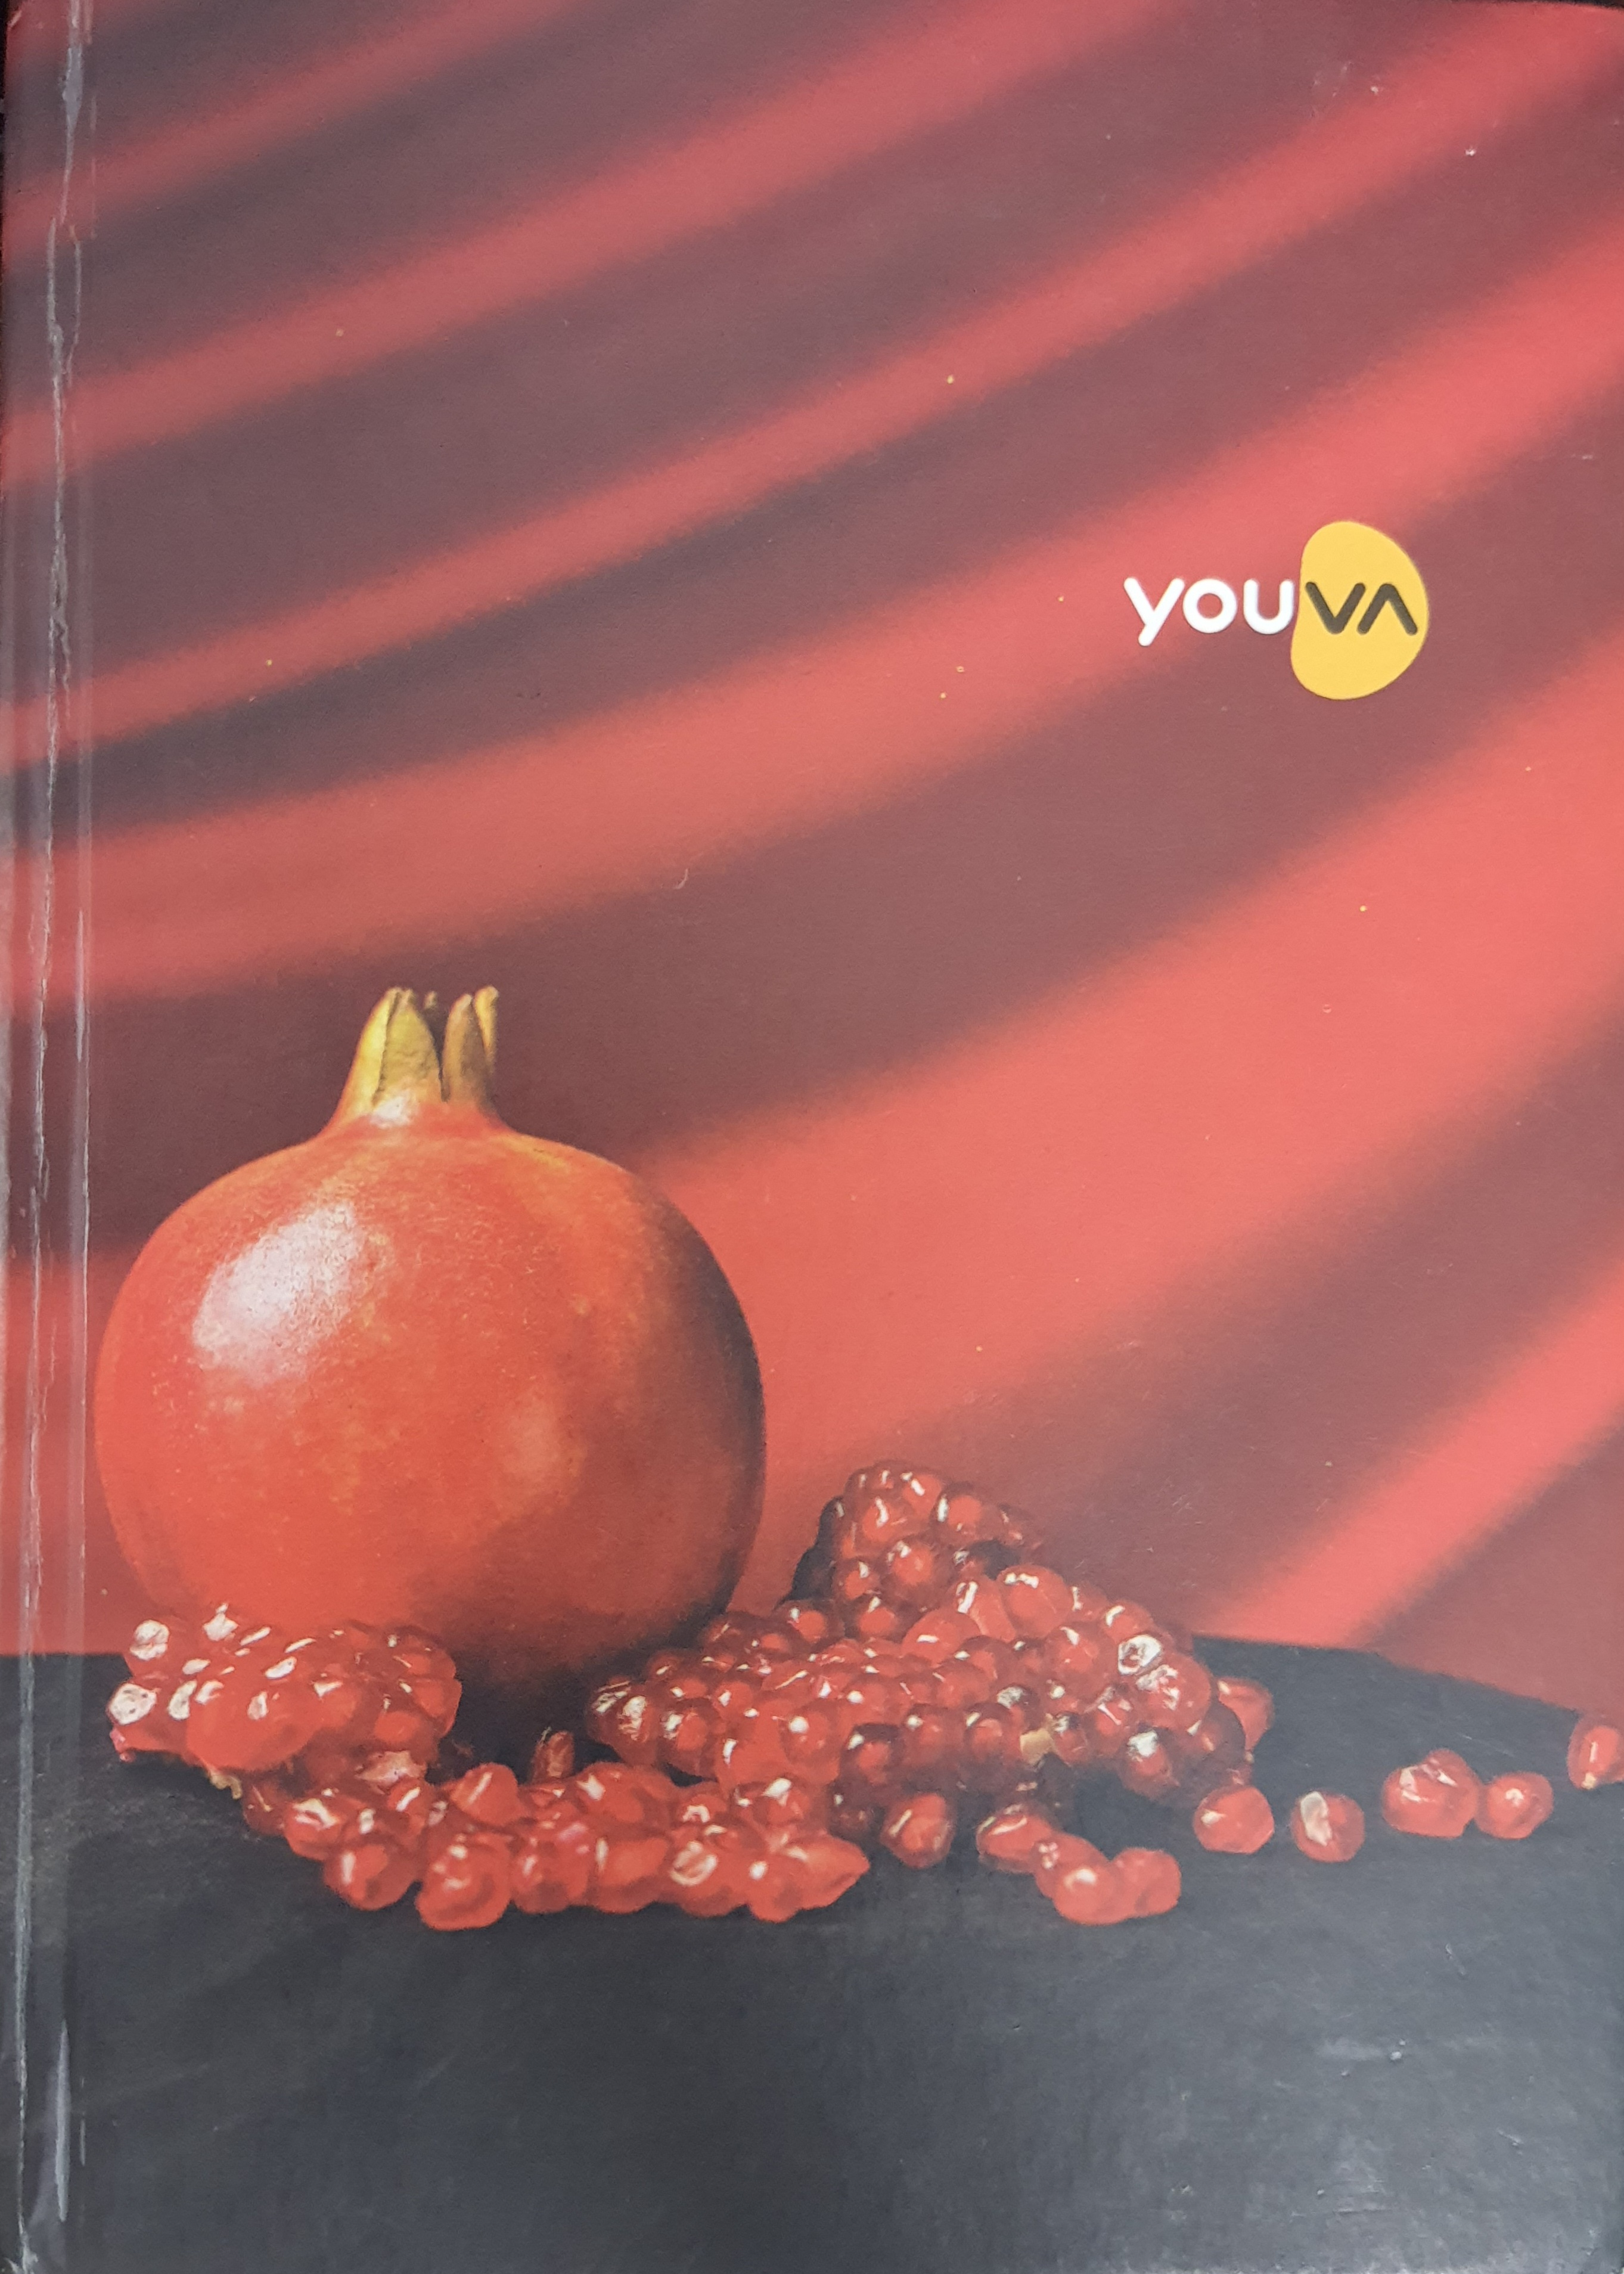
\includegraphics[width=0.46\linewidth]{template.jpg}
    \caption{The isolated red-notebook template. Its pomegranate illustration, logo, edges, and texture provide local features for SIFT.}
    \label{fig:template}
\end{figure}

\section{Method}
The pipeline has six stages. The main program limits each image's largest dimension to 2560 pixels before processing; detections are then mapped back to the original scene coordinates for display.

\subsection{SIFT features}
SIFT is used to detect local keypoints and compute 128-dimensional descriptors for both images \cite{lowe2004sift}. This is the one recognition component delegated to OpenCV \cite{opencv_library}, as allowed by the assignment. SIFT supplies location $\mathbf{p}$, scale $s$, orientation $\theta$, and a descriptor vector $\mathbf{d}$ for every keypoint.

\subsection{Scene-to-template correspondence}
For every scene descriptor $\mathbf{d}_s$, the implementation computes its Euclidean distance to every template descriptor $\mathbf{d}_{t,j}$:
\begin{equation}
    D_j = \lVert \mathbf{d}_s - \mathbf{d}_{t,j} \rVert_2.
\end{equation}
Let $D_1$ and $D_2$ be the smallest and second-smallest distances. A correspondence is retained only when Lowe's ratio test passes:
\begin{equation}
    \frac{D_1}{D_2} < 0.75.
\end{equation}
Matching from scene features to template features is important here because one template feature may legitimately recur across multiple notebook instances. No \texttt{BFMatcher} or \texttt{FlannBasedMatcher} is used.

\subsection{4D Generalized Hough voting}
Each retained correspondence predicts the centre, scale, and orientation of an object instance. If $\mathbf{c}_t$ is the template centre, $\mathbf{p}_t$ is a matched template keypoint, and $\mathbf{p}_s$ is its scene match, then the match predicts
\begin{align}
    r &= \frac{s_s}{s_t}, \\
    \phi &= (\theta_s - \theta_t) \bmod 360^\circ, \\
    \hat{\mathbf{c}}_s &= \mathbf{p}_s + r R(\phi)(\mathbf{c}_t - \mathbf{p}_t),
\end{align}
where $R(\phi)$ is the 2D rotation matrix. This follows the Generalized Hough Transform idea of accumulating pose-consistent local evidence \cite{ballard1981ght}. The tuple $(\hat{c}_x, \hat{c}_y, r, \phi)$ is quantized into a 4D bin. The implementation uses 20-pixel position bins, 0.1 scale bins, and $15^\circ$ orientation bins. Bins with at least three votes become candidates for geometric verification.

\subsection{Affine verification with RANSAC and least squares}
A candidate Hough bin may still include mismatches. RANSAC \cite{fischler1981ransac} repeatedly samples three correspondences, skips collinear template samples, and fits an affine transformation
\begin{equation}
    \begin{bmatrix}x'\\y'\end{bmatrix} =
    \begin{bmatrix}a & b\\c & d\end{bmatrix}
    \begin{bmatrix}x\\y\end{bmatrix} +
    \begin{bmatrix}t_x\\t_y\end{bmatrix}.
\end{equation}
For $n$ correspondences, the six unknown parameters are solved with the least-squares system $A\mathbf{q}=\mathbf{b}$ using \texttt{numpy.linalg.lstsq} \cite{harris2020numpy}; no OpenCV affine-estimation routine is called. A match is an inlier when its Euclidean reprojection error is at most 5 pixels. The best model maximizes the inlier count and, on a tie, minimizes total inlier error. It is then re-fit using all of its inliers.

A final sanity check rejects reflected, singular, excessively scaled, or heavily sheared transformations. In particular, the linear component must have positive determinant, a scale between 0.25 and 4.0, and a condition number no larger than 3.0.

\subsection{Iterative extraction and NMS}
After accepting a model, the four template corners are projected through it. These corners are retained and rendered as an oriented quadrilateral, so the final boundary follows the estimated rotation instead of being forced into an axis-aligned rectangle. Their axis-aligned envelope is additionally stored for IoU-based suppression. The RANSAC inliers are removed from the active match list, then Hough voting and verification repeat to seek another instance. Finally, detections are ranked by their inlier counts and standard IoU non-maximum suppression removes lower-scoring envelopes whose overlap is at least 0.5.

\section{Implementation summary}
Table~\ref{tab:parameters} lists the principal configuration values. They are centralized in \texttt{main.py} to make experiments easier to reproduce.

\begin{table}[htbp]
    \centering
    \caption{Pipeline parameters used for the supplied images.}
    \label{tab:parameters}
    \begin{tabular}{lr}
        \toprule
        Parameter & Value \\
        \midrule
        Maximum SIFT features & 6000 \\
        Lowe ratio threshold & 0.75 \\
        Hough position bin & 20 px \\
        Hough scale bin & 0.1 \\
        Hough angle bin & $15^\circ$ \\
        Minimum Hough votes & 3 \\
        RANSAC iterations & 500 \\
        RANSAC reprojection threshold & 5 px \\
        Minimum RANSAC inliers & 3 \\
        NMS IoU threshold & 0.5 \\
        \bottomrule
    \end{tabular}
\end{table}

\section{Results and discussion}
The updated high-detail configuration uses a 2560-pixel processing limit and a 6000-feature SIFT cap. On the supplied images, it extracted 2070 template keypoints and 6000 scene keypoints; the scene count reaches the configured cap. Lowe's ratio test retained 893 matches. The greedy stage accepted 77 affine hypotheses and accumulated 573 verified inlier matches; IoU NMS reduced these to four final candidate boxes. These are pipeline measurements, not ground-truth accuracy metrics: the scene has not been manually annotated, so precision and recall are deliberately not claimed.

Figure~\ref{fig:naive} visualizes the matches surviving the descriptor-ratio test. Although many lines terminate around real notebook details, the picture remains hard to interpret. Similar colours, repeated pomegranate texture, notebook edges, and general clutter all create plausible local correspondences. This is precisely why nearest-neighbour matching cannot be treated as an object detector.

Figure~\ref{fig:verified} contains only matches retained as RANSAC inliers over the greedy extraction process. Relative to Figure~\ref{fig:naive}, the evidence is more structured, but correspondence overlays still do not communicate the final localization as clearly as oriented boundaries.

\begin{figure}[htbp]
    \centering
    \begin{subfigure}[t]{0.49\linewidth}
        \centering
        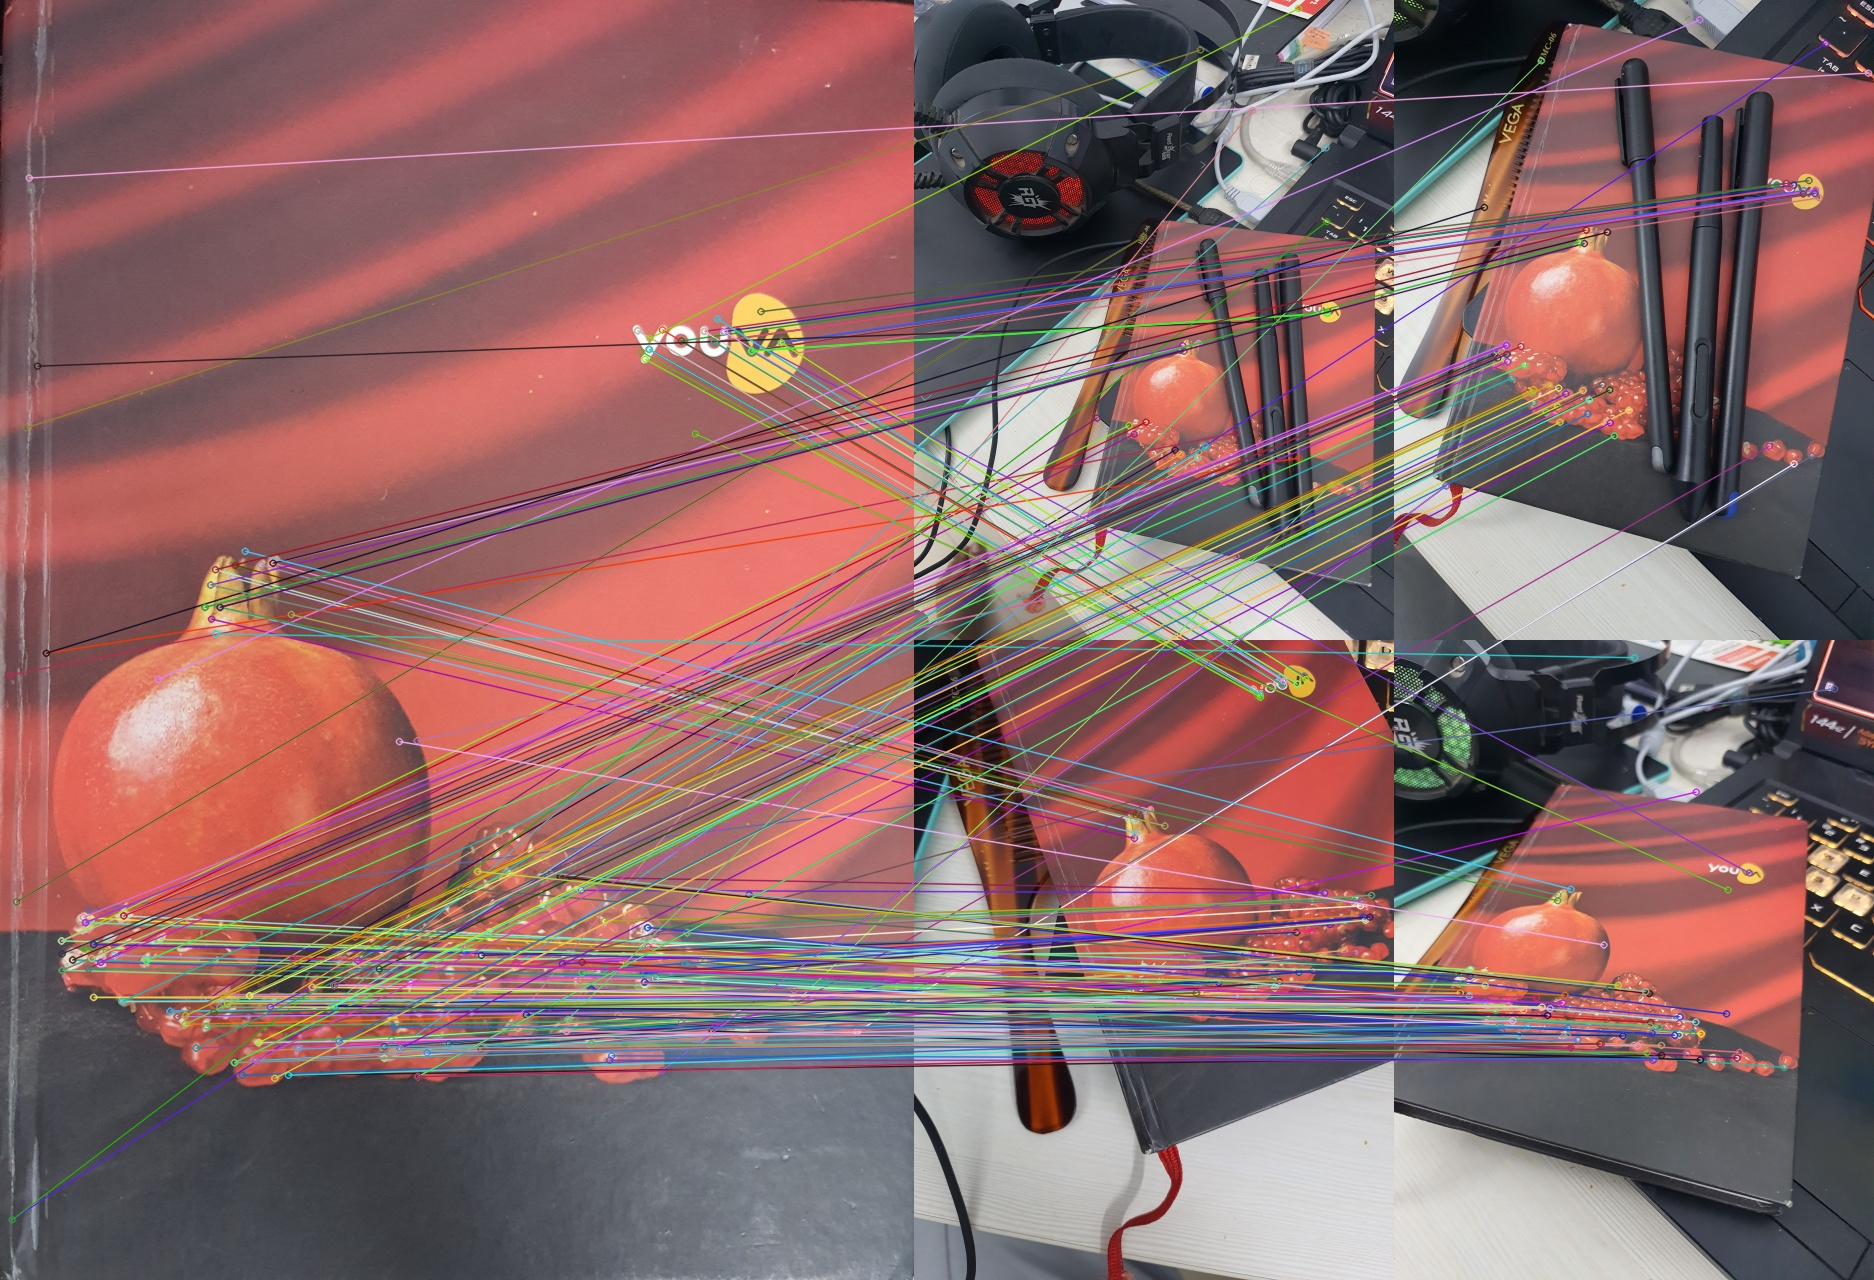
\includegraphics[width=\linewidth]{naive_matches.jpg}
        \caption{Naive ratio-test matches.}
        \label{fig:naive}
    \end{subfigure}
    \hfill
    \begin{subfigure}[t]{0.49\linewidth}
        \centering
        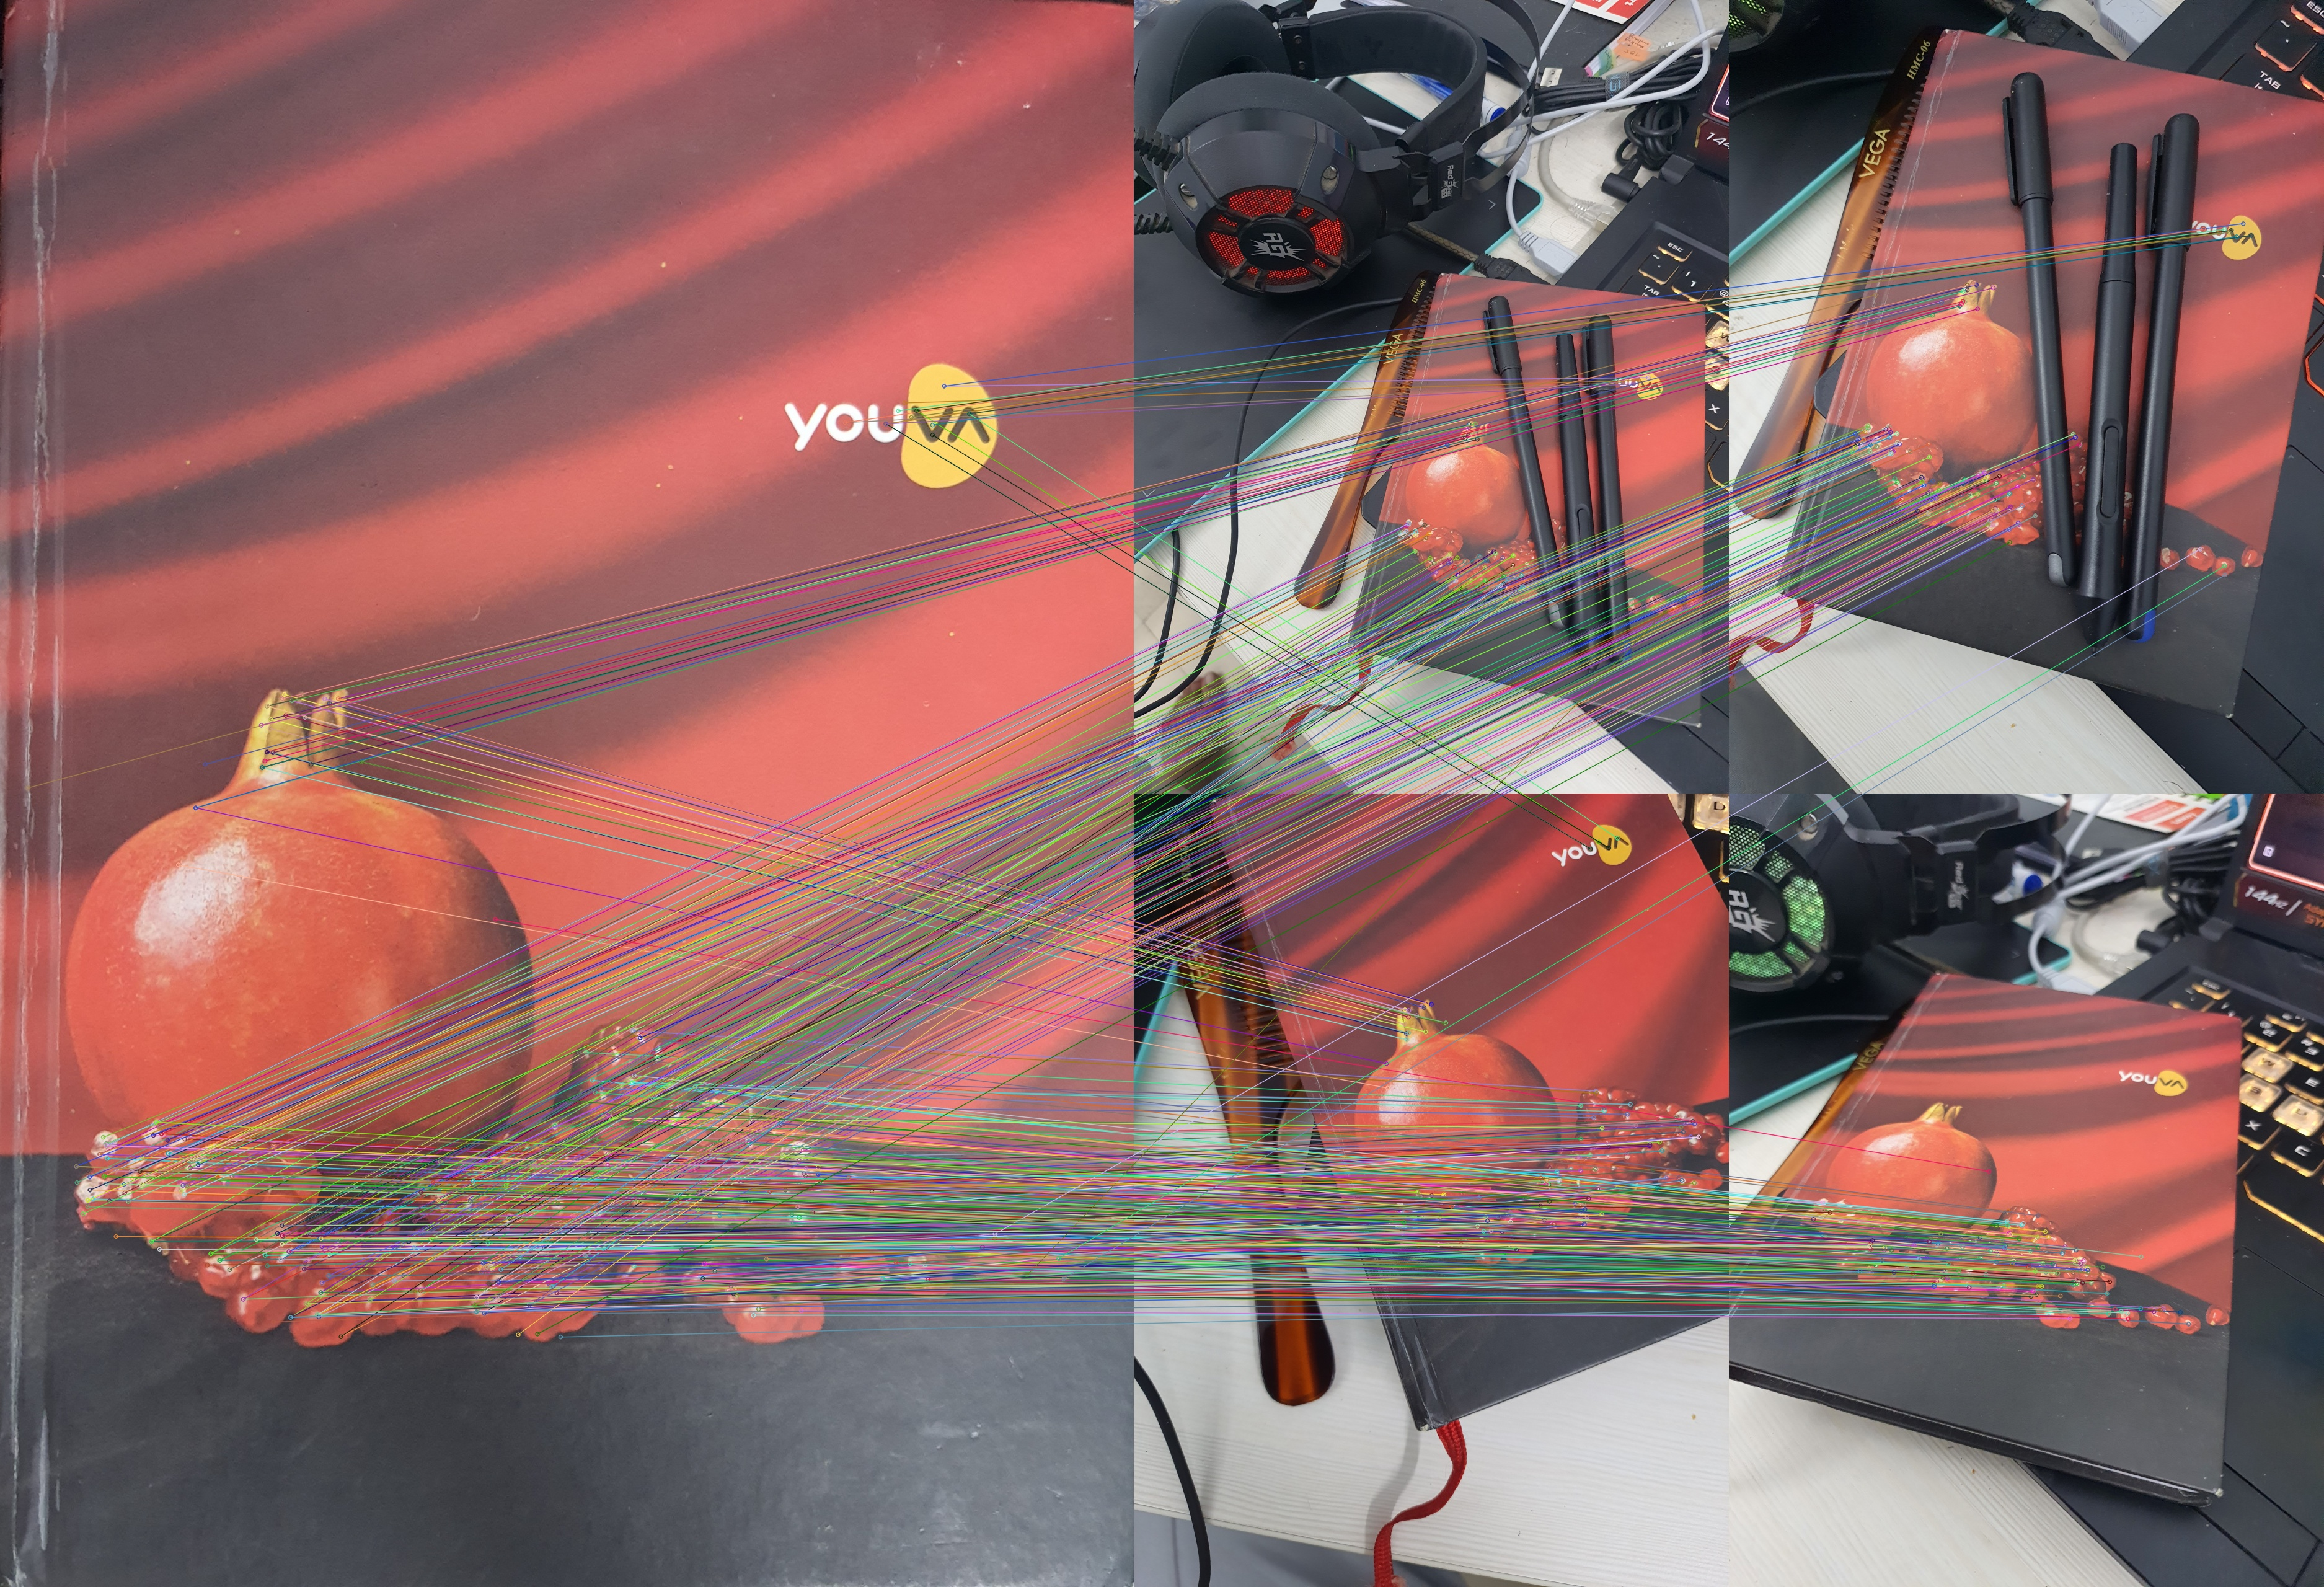
\includegraphics[width=\linewidth]{verified_matches.jpg}
        \caption{RANSAC-verified inlier matches.}
        \label{fig:verified}
    \end{subfigure}
    \caption{Match refinement. The ratio test removes ambiguous nearest-neighbour matches, while Hough clustering and affine RANSAC retain evidence that agrees on a common object pose.}
    \label{fig:match-comparison}
\end{figure}

The final output in Figure~\ref{fig:final} is much easier to read than the raw match overlay. It places oriented quadrilateral boundaries on notebook instances across different rotations and scales. However, it also retains candidate boxes that do not cleanly correspond to a notebook. The headset and large regions of background are particularly challenging. Therefore, the correct interpretation is not ``perfect detection'' but a substantial reduction of noisy matches into a small, inspectable set of hypotheses.

\begin{figure}[htbp]
    \centering
    \includegraphics[width=0.68\linewidth]{final_detections.jpg}
    \caption{Final oriented outlines after affine verification, greedy extraction, and IoU non-maximum suppression. Each green quadrilateral is the template's four corners projected by its affine model; candidates are scored by RANSAC inlier count. Some false positives remain in this highly cluttered scene.}
    \label{fig:final}
\end{figure}

\section{Limitations and next steps}
The experiment exposes expected limits of a local-feature pipeline. First, a three-vote minimum is intentionally permissive and can allow weak Hough clusters through RANSAC. Raising the minimum vote or inlier requirement would likely remove some false positives, although it might also miss a more occluded notebook. Second, the final NMS uses axis-aligned boxes, while the physical notebooks are rotated; polygon-aware overlap could better express duplicate detections. Third, the affine model is a pragmatic approximation. A projective model could handle stronger viewpoint changes, but it would require more correspondences and a different estimator.

Useful next experiments are to sweep the ratio, vote, and reprojection thresholds; report precision and recall against hand-labelled boxes; and inspect detections at each parameter setting. These changes would turn the present qualitative evaluation into a more systematic comparison without changing the core idea of grouping local evidence before fitting geometry.

\section{Reproducibility}
From the repository root, run:
\begin{verbatim}
uv sync
uv run python main.py
\end{verbatim}
The script reads \texttt{data/template.jpg} and \texttt{data/scene.jpg}, then creates the three images used above in \texttt{outputs/}. RANSAC is initialized with seed 42, so its sampled hypotheses are repeatable for a fixed software environment. The complete source is organized by pipeline stage in \texttt{src/}; the project README provides a concise map of the files and available settings.

\clearpage
\begin{thebibliography}{9}

\bibitem{lowe2004sift}
David G. Lowe.
\newblock Distinctive image features from scale-invariant keypoints.
\newblock \emph{International Journal of Computer Vision}, 60(2):91--110, 2004.
\newblock \url{https://doi.org/10.1023/B:VISI.0000029664.99615.94}

\bibitem{ballard1981ght}
Dana H. Ballard.
\newblock Generalizing the Hough transform to detect arbitrary shapes.
\newblock \emph{Pattern Recognition}, 13(2):111--122, 1981.
\newblock \url{https://doi.org/10.1016/0031-3203(81)90009-1}

\bibitem{fischler1981ransac}
Martin A. Fischler and Robert C. Bolles.
\newblock Random sample consensus: A paradigm for model fitting with applications to image analysis and automated cartography.
\newblock \emph{Communications of the ACM}, 24(6):381--395, 1981.
\newblock \url{https://doi.org/10.1145/358669.358692}

\bibitem{opencv_library}
OpenCV Team.
\newblock OpenCV: Open Source Computer Vision Library.
\newblock \url{https://opencv.org/}

\bibitem{harris2020numpy}
Charles R. Harris et al.
\newblock Array programming with NumPy.
\newblock \emph{Nature}, 585:357--362, 2020.
\newblock \url{https://doi.org/10.1038/s41586-020-2649-2}

\end{thebibliography}

\end{document}
